\subsection*{Direct PET Image Reconstruction Incorporating Deep Image Prior and a Forward Projection Model}
% \subsection*{Ссылка} \url{https://arxiv.org/abs/2109.00768}
\subsubsection*{Введение}
Для того, чтобы снизить уроень радиации, поглощаемый пациентом при обследовании, 
проводят ПЭТ-визуализацию с низкими дозами облучения, что в свою очередь негативно влияет на 
зашумленность изображения. Существуют различные методы по постобработке ПЭТ-изображений,
такие как шумоподавление и восстановление для улучшения качества снимков при распознавании 
малых образований и количественном анализе. В данной работе \cite{ann9} предлагается метод
прямого восстановление ПЭТ-изображения, включающий в себя DIP фреймворк.
Алгоритм включает в себя модель прямой проеккции в функции потерь, чтобы достичь 
прямой реконструкции ПЭТ-изображения из синограм без учителя. 
\subsubsection*{Основная идея}
Модель прямой проекции ПЭТ может быть выражена так, что проектируемые данные \(y\in\mathbb{R}^{Mx1}\) связаны 
с пространственным распределением радиоактивного индикатора \(x\in\mathbb{R}^{Nx1}\) посредством афинного 
преобразования \(y=Px\), где \(P\in\mathbb{R}^{MxN}\) - матрица проекции, которая 
отражает вклад каждого вокселя в каждую линию ответа (line of response, LOR).
Реконструируемое изображение \(x\) вычисляется с помощью DIP фреймворка
следующим образом: \(x=f(\Theta|z)\), где \(f\)- это CNN, \(\Theta\) - веса CNN, а 
\(z\) - предыдущий входной вектор CNN. В данной работе для вычисления реконструированного 
изображения напрямую предлагается модель прямой проекции \(P\), втсроенная в функцию потерь. Была 
использована модель, основанная на 3D UNet и адаптированная под текущую задачую

\begin{minipage}{1.0\linewidth}
    \begin{center}
        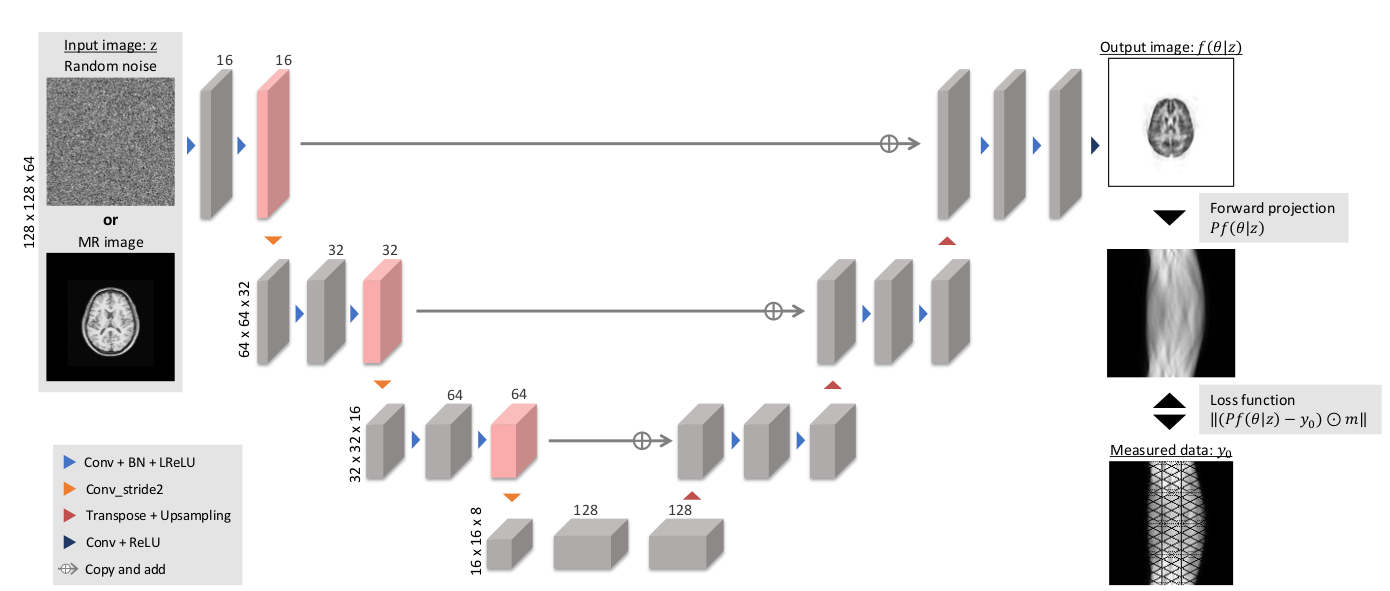
\includegraphics[scale=0.3]{ann9_arch.png} \\
        \captionof{figure}{\scriptsize{Общий вид предложенной модели прямой реконструкции ПЭТ.}}
    \end{center}
    
\end{minipage}

\subsubsection*{Данные} BrainWeb и созданные данные по методу Монте-Карло.
\subsubsection*{Результаты}
Был проведен сравнительный анализ предложенного метода
с методом filtered back projection (FBP) с использованием фильтра 
Ханна и Гаусса, а также с методом ML-EM. Показано, что описанный в статье метод
используя случайный шум и МРТ-изображение точно реконструирует ПЭТ-изображение 
без сокрытия или потерь информации в сравнении с методами FBP и ML-EM.
Основное ограничение данного исследования состоит в том, что оценивался 
только датасет ПЭТ изображений, полученных с радиоактивной меткой ФДГ.

\begin{minipage}{1.0\linewidth}
    \begin{center}
        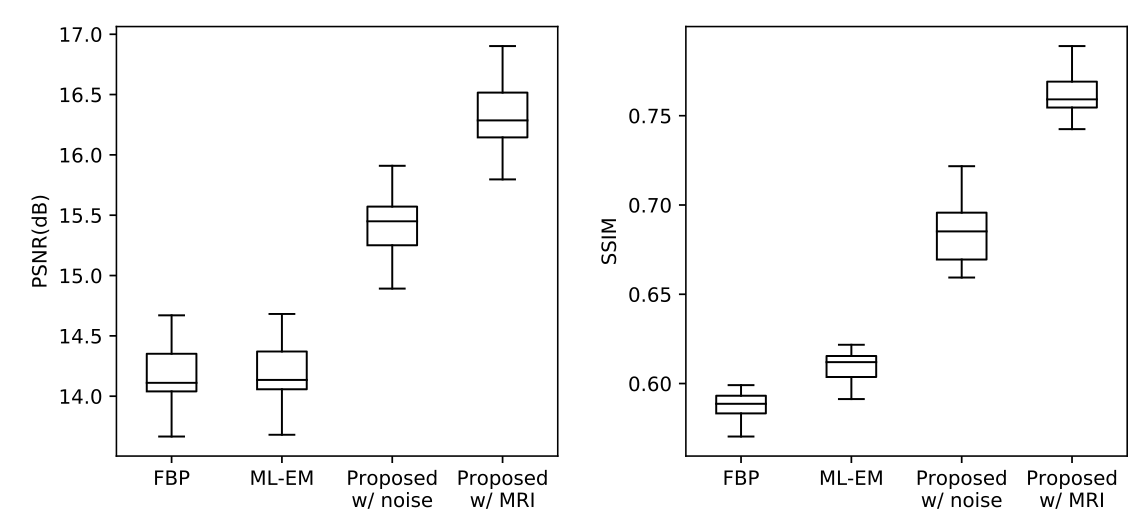
\includegraphics[scale=0.3]{ann9_res.png} \\
        \captionof{figure}{\scriptsize{Количественные результаты реконструированных
        изображений по метрике PSNR(слева) и SSIM(справа) относительно различных алгоритмов.
        Линия внутри прямоугольника представляет медиану, верхние и нижние линии прямоугольника - 
        75-й и 25-й перцентили соответственно. Верхние и нижние \glqq антенны\grqq представляют максимум и минимум соответственно.
        }}
    \end{center}
    
\end{minipage}
\subsubsection*{Заключение}
В сравнении с традиционными алгоритмами FBP и ML-EM, предложенный
метод показал лучший результат по метрикам PSNR и SSIM на данных, смоделированных с
использованием ФДГ.